\documentclass[]{article}

\usepackage{graphicx, wrapfig}
\usepackage{float}
%opening
\title{Theft Tracker: A Localization Algorithm to Track Position of Stolen Vehicles using WSN}
\author{Giorgio Cozza (CP:10649461, MAT:904965)}

\begin{document}

\maketitle

\section{Problem}

GPS is one of the most popular technology for object localization around the earth, usually employeed by car antitheft systems to localize stolen vehicles. Unfortunately in most of the cases such kind of service is subjected to a fee that customers do not consider convenient especially for vehicles without the sufficient technology to support it. 
Theft Tracker tries to overcome this limitation by using sensor nodes located on vehicles to broadcast alert messages to the neighbour nodes in case the car gets stolen and the traffic is then broadcasted by the receivers until a \textbf{network gateway} is reached. Such type of mote provided with GPS uses a rough estimation of the distance from the origin that sends together with its coordinates to the server.


\section{Solution}

\begin{wrapfigure}{r}{5.5cm}
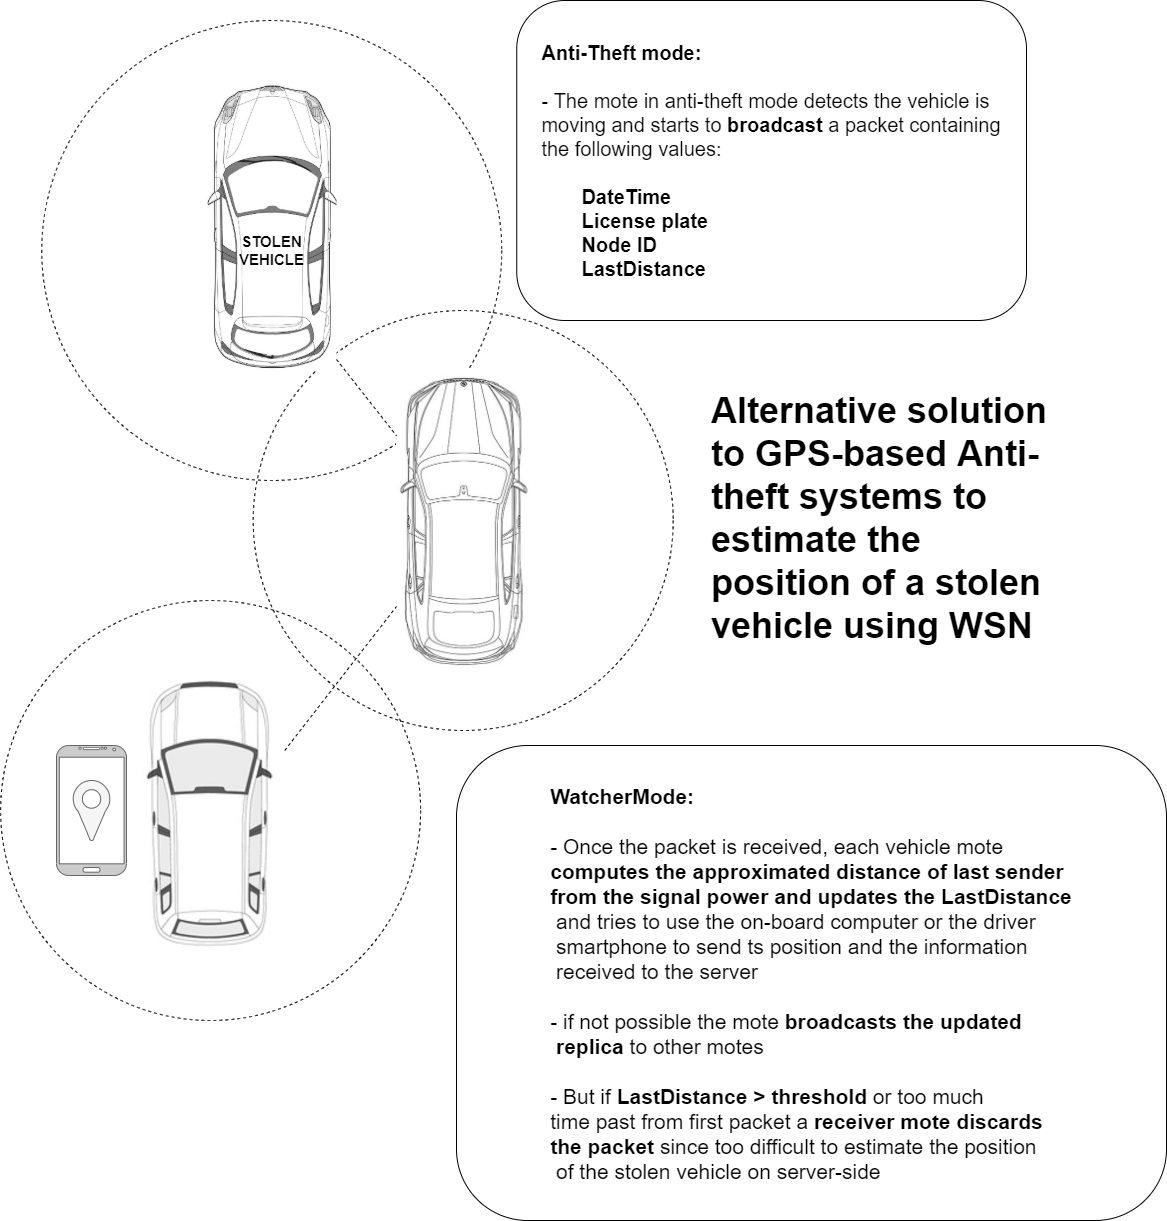
\includegraphics[width=7.5cm]{./images/theft_tracker_summary.png}
\caption{Theft Tracker summary.}\label{wrap-fig:1}
\end{wrapfigure}

\subsection{Mote Application}

The application conceived for constrained sensor nodes runs on Contiki OS. Two different programs are developed, one for the simple mote in charge of broadcasting alert messages received from the stolen vehicle or from other motes (\textbf{ttmote}) and one for the network gateway (\textbf{ttgateway}) that wraps the GPS coordinates together with a distance estimation from the origin and sends such data to the server. The information exchanged by the ttmotes includes:
\begin{itemize}
	\item first mote ID: an identification number of the alert origin
	\item event clock time: the number 
	\item <third>
	\item <fourth>
\end{itemize}


\end{document}
